\documentclass[llncsdoc]{llncs}
\usepackage[latin1]{inputenc}
\usepackage{epsfig}
\usepackage{epstopdf}
\usepackage{graphicx}
\usepackage{makeidx}
\usepackage{subfigure}
\usepackage{multirow}
\usepackage{indentfirst}
\usepackage[printonlyused]{acronym}
\usepackage{booktabs}
\usepackage[table]{xcolor}
\definecolor{lightgray}{gray}{0.9}

\usepackage[table]{xcolor}
\usepackage{array}
\usepackage{url}
\newcolumntype{P}[1]{>{\centering\arraybackslash}p{#1}}
\begin{document}
\pagestyle{plain}
\makeatletter
\renewcommand\subsubsection{\@startsection{subsubsection}{2}{\z@}%
	{-18\p@ \@plus -4\p@ \@minus -4\p@}%
	{8\p@ \@plus 4\p@ \@minus 4\p@}%
	{\normalfont\normalsize\bfseries\boldmath
		\rightskip=\z@ \@plus 8em\pretolerance=10000 }}
\DeclareRobustCommand{\rchi}{{\mathpalette\irchi\relax}}
\newcommand{\irchi}[2]{\raisebox{\depth}{$#1\chi$}}
		
\title{Reputation Vault}


\author{João Santos\\joao.marques.santos@tecnico.ulisboa.pt}
\institute{Instituto Superior T�cnico\\(Advisors: Professors Nuno Santos and David Dias)}
\maketitle
\thispagestyle{plain}


\begin{abstract}

  Something about this
\end{abstract}

\section{Introduction}

\subsubsection{Understanding Reputation}
%what is reputation?%
Reputation lies on the principle that past actions are a good indicator of future behaviour and can be useful to help a party decide whether to trust another one.
While in the past reputation was closely related to the word of mouth, in the sense that people would just talk to each other in order to know information about a given subject, nowadays in the digital age that reality is shifting more and more towards highly sophisticated reputation systems and mechanisms that live in digital platforms. These systems can be centralised or distributed, \cite{Anonymous:6b33pOF-}. Centralised reputation systems collect reputation information (evidence) from the system's user base, aggregate that information and compute, for each user, a reputation score that is then made publicly available. One of the shortcomings of this type of systems is the reputation evidence they collect can not be used by other reputation systems, creating what if called a silo or walled garden. It is easy for one to imagine a scenario where a seller's reputation on eBay could be useful if that same seller was creating an Amazon account. Besides not being able to share reputation information with other systems, another underlying problem of centralised reputation systems is that they have full control over a subject's reputation. That means that if the system's owners ever decide to stop the service, one's entire reputation vanishes.
On distributed reputation systems, on the other hand, there is no centralised platform aggregate the collected evidence, so they either use a distributed database to store information about past interactions or nodes directly query each other when they want information about a given user and make decisions regarding establishing trust with that node.
Examples of centralised reputation systems are the ones implemented on e-Commerce platforms such as Amazon and eBay that help buyers and sellers to establish relationships of trust, advice platforms (such as Yelp or Stack Overflow), ride-sharing (Uber, Cabify) or house renting (AirB\&B).
An example of a distributed reputation system is the one operating on the P2P file-sharing platform Gnutella. This system is designed to disincentivise free-loaders (users who only download and do not upload).
Each of these platforms implements their reputation system according to different rules and to serve different purposes. eBay uses one of the simplest forms of reputation score computation, the Simple Summation algorithm where the reputation score is the difference between the number of positive and negative interactions. Amazon takes this a step further by using an Average Reputation rating system, which accounts for more sophisticated metrics a weighted average, attributing different weights to different reviews based for instance on the reputation of the reviewer or age of the review.
An even more advanced model is the Multinomial Bayesian Reputation System. It allows for different level ratings, which is very useful for distinguishing between cases of polarised and average ratings.

Just like any other digital information system, Reputation Systems can also be the target of attacks. \cite{YanSun:2017jb} provides models to classify and mitigate the various possible attacks. One of the pathways towards mitigating many of the attacks' reputation systems can be targeted with pairing the reputation system with a strong identity system, which among other things should have a mechanism to prevent an individual from creating several identities, \cite{Hoffman:2009gm}.

\subsubsection{Blockchain}
Blockchain technology was made popular with the creation of the Bitcoin \cite{Anonymous:JOJGrvgg}, in 2009. Bitcoin was the first truly decentralised crypto-currency, it uses cryptographic properties to solve the Double-spending problem and allows for parties to engage in transactions without having to trust each other. On backbone of Bitcoin is the blockchain which is a distributed ledger that keeps track of every valid transaction that ever took place in the network. Transactions are validated and packed into blocks that are then added to the ledger by nodes (miners) that run a consensus protocol, proof-of-work in the case of Bitcoin. Bitcoin's blockchain has full auditability \footnote{meaning that any node can verify the validity of any transaction} and correctness \footnote{meaning that all the transactions on the longer chain are valid}.

Following Bitcoin's success, a large and active community has emerged and worked on a lot of modifications and extensions to the original protocol to improve some of Bitcoin's shortcomings like performance, introduce new consensus protocols, add new features. These modifications and extensions, which are usually forks of Bitcoin or abstractions that sit on top of existing blockchains, are called "alt-coins", \cite{Bonneau:2015ema}.

// // Aqui falar mais sobre alt-coins // //

One of the shortcomings of Bitcoin was the lack of contract customisation as while it did allow for parties to create some rules regarding a given transaction (such as requiring a third party to approve the transaction) doing so required learning a not very intuitive scripting language and functionality was extremely limited. In other words, it only allowed for a very simple form of smart contracts \footnote{smart-contracts are programs that run on the blockchain and allow for the creation of special transaction rules}. Ethereum is a crypto-currency blockchain, similar to Bitcoin in many ways, that is a smart contract and decentralised application platform. It has a Turing complete programming language which allows for users to create distributed applications while making use of the features of the blockchain.

\subsubsection{Where Reputation and Blockchain Meet}
Blockchains such as Bitcoin or Ethereum are truly decentralised systems that ensure correctness. They can not be controlled by one single party and all the state transitions they store can be audited by any node. Ethereum's smart contracts and programmability features can be leveraged to create a decentralised reputation system that provides the same functionality as current systems, such as eBay's or LinkedIn's, while solving the information silo problem. It allows for each node to have control over its identity and know that the system will never cease to exist. There are currently some blockchain reputation systems that aim at doing this, \cite{Dennis:2016um}, \cite{Yasin:2016ja} and \cite{Buechler:2015tv}. At the same time, communities have formed pursuing efforts in this field, like Rebooting The Web of Trust and IDEO CoLab's Mosaic, that focuses mainly on identity.



\section{Goals}
\label{sec:goals}

This project serves one purpose.
 
\begin{quotation} 
\textit{Goals:} To create an amazing system.
\end{quotation} 
 
\begin{quotation} 
  \textit{Expected results:} Be hired by and become best friends with Elon Musk.
\end{quotation} 

\section{Related Work}
\label{sec:rwork}

\subsubsection{Types of Reputation Systems}
Centralised vs distributed
Reputation Algorithms



\subsubsection{Identity and Reputation}
One of the keys to having a good reputation system is having a strong identity framework put in place. As we are going to see later, many of the deficiencies of current reputation systems originate in poor identity verification mechanisms operating on the backbone of said reputation systems. It is essential to ensure that one person is linked to one and only one identity.

\subsubsection{Silos and Walled Gardens}
Many of the identity and reputation systems (Google, Facebook, Amazon) we use today are extremely atomic in the sense that the information collected by each one is not shared, or even compatible, to the one that is stored in other systems. What this creates, for each user, is a set of incomplete identities. Each platform only looks to a subset of features of a user and that prevents it from creating a holistic picture of him. In places like Amazon and eBay we have what is called an identity silo \cite{Pato:2017uw}, where the information in centralised and controlled by one entity without the possibility of being interchanged with another platform that might serve a similar purpose. Google and Facebook also started off as being identity silos, but now with the single sign on features \cite{Anonymous:MGy1lR79} they became what are known as Walled Gardens \cite{Pato:2017uw}, which are like Silos but that allow some information to be shared with some other organisations. \cite{Anonymous:PvP3cFwB} and \cite{Mostarda:2009te} suggest a solution to part of this problem in the form of a social network's social graphs aggregator. 

\subsubsection{Reputation Systems Attacks and Vulnerabilities}
\cite{Hoffman:2009gm} suggests a classification of these attacks in five categories. 
\begin{itemize}
     

\item Self-promoting, where attackers falsely increase their own reputation
\item Whitewashing, where attackers leverage system vulnerabilities to repair their reputation, effectively giving themselves a clean slate to continue engaging in malicious behaviour.
\item Slandering, where attackers lower other users' reputation score by illegitimately (without having existed an interaction) rating them.
\item Orchestrated, where several attackers collude to carry on one of the attacks described above.
\item Denial of service, where attackers prevent the calculation and dissemination of reputation scores thus compromising the normal function of the system.
\end{itemize}

\subsection{Bitcoin}

\subsubsection{Historical Context}

 Since the 1980's that there had been proposals for crypto-currency systems and in 2005 for decentralised consensus protocols. The proposed crypto-currency systems were never widely adopted due to the need of a centralised platform, as for the decentralised consensus protocols, they never became a reality as it was unclear how to carry out the implementation.
 Bitcoin's white paper,\cite{Anonymous:JOJGrvgg}, was published in 2009 by Satoshi Nakamoto (a pseudonym) and it was the first successful implementation of a decentralised cryptocurrency system.
 
 The technical breakthrough it provided was the implementation of a blockchain, a distributed ledger that keeps track of transactions. 
 \subsubsection{Technical Breakthrough}
 Bitcoin proposed an alternative mode of establishing trust between transacting parties. On traditional financial transaction systems, such as banks, two transacting entities have trust on a centralised element, the bank. Let us look at the example of a normal wire-transfer. User A sends money to user B. Both A and B are confident that the bank will withdraw the right amount of money from A's account and place that same amount in B's account. In this traditional trust model the bank is an essential entity in the process as it constitutes the only source of trust between the two transacting parties. Bitcoin's approach is different. Instead of asking the two parties to trust each other, it uses a proof-of-work system whose cryptographic properties are enough to assure transactional correctness as long as honest nodes control the majority of the CPU power of the network.
 
 An electronic currency is nothing more than a piece of digital data and one of the features of digital data is their easy replication. For that reason, an issue that an electronic currency has to tackle is the double spending problem. That is, ensuring that a given node is not able to spend the same token\footnote{coin, a unit of digital currency} more than once. The way to solve this problem without resorting to a centralised system is to create a ledger of transactions and get all the nodes to agree on the content of that ledger. 
 To that end, a consensus protocol is used, the Bitcoin consensus protocol, also known as the Nakamoto Consensus if based on a proof-of-work.
 
 \subsubsection{Transactions and Proof-of-Work}
 A Bitcoin transaction consists on nodes exchanging unspent coins and is identified by chain of digital signatures. To complete a transaction the sending node digitally a hash that identifies the past transaction and the public key of the next owner. This ensures that each transaction is linked to the ones preceding it, creating a chain.
 The next key challenge is getting all the nodes to agree on the set of past transactions, in order to prevent double-spending.
 To that end transactions are packed into blocks, and added to an append-only data structure, the blockchain.
 
 To add a block to the blockchain, nodes have to mine the block and the way to do that is to solve a mathematical challenge with a pre-defined difficulty level. The first node to solve that challenge mines the block, permanently adding it to the Blockchain. Each time a node mines a block, a new Bitcoin (coin) is created and given to that node. This constitutes an incentive for nodes to mine. The algorithm is designed to automatically adjust the challenger's difficulty in order to regulate the currency issuing rate.
 
 All the mined blocks are made of transactions that are linked to each other, which means that if a dishonest node was to change a past transaction that change would be eventually be detected by an honest node.
 
 
\subsubsection{Solving Forks}
Sometimes a node will mine a block that has already been mined by another node but due to network latency the first is unaware of this. In this situation a fork occurs. Both of these blocks are propagated through the network and eventually a new block will be mined and appended to one of those forks. The network will chose the longest fork as the standing one.
 
\subsection{Alt-coins}

\subsection{Ethereum}
Ethereum is built on many of the same principles as Bitcoin. Is is a blockchain based system that can also serve as a cryptocurrency. It also uses a proof-of-work mechanism as consensus protocol, albeit with a difference, while Bitcoin's consensus protocol challenge lies on CPU power, Ethereum's lies on memory requirement. The goal of this different implementation is to make the network more democratic. One of the consequences of Bitcoin's consensus protocol was the creation of mining farms\footnote{Infrastructures provided with bitcoin mining specialised hardware} which resulted on an uneven distribution of the mining power among active nodes. Memory is something that is extremely optimised on pretty much every electronic device nowadays, much more than CPU power, so this measure should empower lighter miners to the detriment of more powerful ones.  


\subsubsection{Rebooting the Web of Trust}
\begin{itemize}
    \item bitkariero
    \item Portable Reputation Kit
\end{itemize}

\subsection{Reputation Systems on the Blockchain}

There are already some attempts of implementing Reputation Systems by making use of the benefits of the Blockchain.
\subsubsection{TURS - User Reputation System}
TURS, \cite{Yasin:2016ja}, proposes a holistic approach to reputation, its goal is to attribute a reputation score to a person. To that end, they present framework that aggregates a person's online social network profiles, personality and professional records. This evidence is collected in different ways. The data regarding social network should be provided by the user, by authorising the system to access its accounts (Facebook, email, etc). Evidence regarding personality is collected via the form of a standardised psychological personality test (when the user joins the network) and via friends and verified friends and family accounts. Finally, to calculate the professional reputation they look at a user's skills (verified by colleagues), degree, publications, citations, certifications and academic followers. The authors do not go into a lot of detail as to how the evidence is actually collected, a more high-level approach is thus provided.
They then feed the collected evidence into an algorithm that outputs a reputation score. 

The reputation score and all of this evidence are associated with an identity. The identity they refer to is a Blockchain ID, which essentially means that one's identity is associated with a public key. While this is enough to identify an individual, it is not enough to stop him from creating multiple accounts and carry on sophisticated reputation system attacks, as \cite{YanSun:2017jb,Ciccarelli:2011gf,Hoffman:2009gm} show. 

\subsubsection{Rep on the Roll}
Rep on the Roll, \cite{Dennis:2016um}, proposes a reputation system for P2P. The evidence collected is user feedback provided after a transaction between two parties. The proposed solution is a new blockchain that runs smart-contracts. The way this smart-contract works is it intermediates a transaction between two parties, guaranteeing that one party asked for a piece of data and that the other party sent it to him. The contract is complete when, upon receiving the data, the party that asked for it rates the sender as to the quality of the data they sent.

One innovative feature of this system is that the burden of calculating the reputation is placed on the enquirer. This means that for a given user, there is not a public value of their reputation score. Each user's reputation score is calculated by the users enquiring that user's reputation. This allows for users to personalise the reputation score algorithm thus creating results that are more relevant to them. 

\subsubsection{Decentralised Reputation System for Transaction Networks}
One more example... Outro Paper

\subsubsection{BitKariero}

\subsubsection{Verity}

\section{Proposed Solution}
Our solution aims to replicate and extend some of LinkedIn's functionality and is going to be based on a merger of concepts that come from BitKariero and Verity and our contributions are as follows:
\begin{itemize}
    \item Add endorsement features to BitKariero
    \item Reduce computing power required by Verity
    \item Compare performance of this system with a centralised one.
\end{itemize}
We propose a skill reputation system based on endorsements and certificates. Its goal if to allow entities to endorse, be endorsed by, or give certificates to other entities on skills they may have. An entity's reputation is derived from the endorsements and certificates it receives over time.
The functionality of this system is very similar to the one provided by LinkedIn's skills endorsement feature. It will support the following tasks:
\begin{itemize}
    \item \textbf{Endorse:} Entities will be able to endorse each other on a number of skills;
    \item\textbf{Issue a certificate:} Entities with a certain reputation score on a given skill will be able to issue certificates;
    \item \textbf{Query:} Entities will be able to query the system for other entities skill reputation scores.
\end{itemize}
The difference lies in the implementation. While LinkedIn's solution is implemented as a centralised system, where one entity (LinkedIn) has total control over the system, ours will be a truly decentralised system, made possible by blockchain technology.
To better understand the system's operation mode, let us consider the scenario presented in Fig.\ref{fig:basic1}. We have three entities A, B and C. In this scenario A is endorsing B on a certain skill and C is consulting B's history.

\begin{figure}
  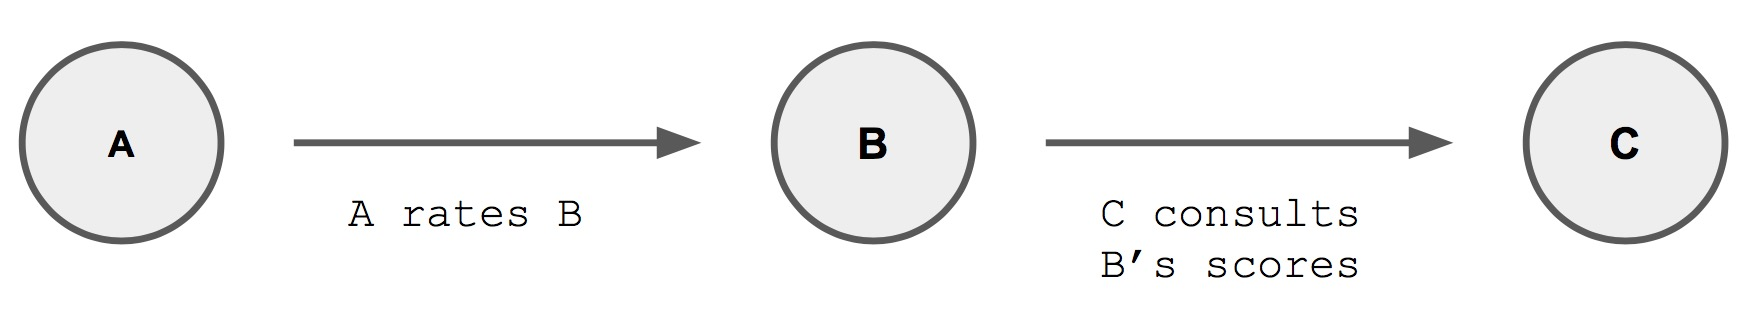
\includegraphics[width=\linewidth]{images/basic_scenario.jpg}
  \caption{Example of usage scenario. A rates B and C consults B's reputation score}
  \label{fig:basic1}
\end{figure}

\subsection{Entities}
Entities is the term used to identify the system's participants. Entities can be single users or groups of users. Each user will have an identity associated to it. That identity is identified by a public key.

\subsection{Certificates and Endorsements}
Endorsements and certificates serve a similar purpose in the sense that they both contribute to an entity's reputation, however they have different properties.

\subsubsection{Certificates}
Certificates are digitally signed documents that an entity can issue to another. It's content can be arbitrary, in the sense that they need not obey a strict format and the receiving entity has control over its privacy. This means that certificates are private documents that can be shared upon request.

An example of a certificate would be a University that gives a diploma to a student who completed a certain degree. That certificate (the diploma in this case) would be annexed to that student's identity, however its content would be private. Any entity can ask the student for permission to view the certificate and for each case the student can decide whether to show, or not show the certificate.

\subsubsection{Endorsements}
Unlike certificates, endorsements are public and exist under a more restrict format. Entities can endorse each other on various skills. The name of the skills itself is not subject to any rule, a skill is therefore simply a label with an arbitrary name. Entities can endorse other entities on existing skills or chose to create new ones.

\subsubsection{Issuing Certificates and Endorsements}
Endorsements and certificate emissions can be made by one of two ways, via a push or pull method.
\begin{itemize}
    \item Pull: An entity asks another entity for an endorsement or certificate .
    \item Push: An entity takes the initiative of sending another user an endorsement or certificate.
\end{itemize}


\subsection{Use Scenarios}
\begin{itemize}
\item \textbf{University Diploma:} Upon completion of a college degree, the university, A, would issue a certificate stating that B had successfully completed such degree.
\item \textbf{Workshop:} Let's assume that A is a photographer and B is a group of participants who attended a photography workshop lectured by A. Upon completion of the workshop, A gives B a certificate stating that B has successfully completed the workshop and now has a new set of skills. At the same time each user in B can endorse A on its skills as a professor.
\end{itemize}






\section{Evaluation}
\label{sec:evaluation}


\subsection{Performance Evaluation}

\section{Scheduling of Future Work}
\label{sec:fwork}

Future work is scheduled as follows:

\begin{itemize}
\item January 9 - March 29: Detailed design and implementation of the
 proposed architecture, including preliminary tests.
\item March 30 - May 3: Perform the complete experimental evaluation.
\item May 4 - May 23: Write a paper describing the project.
\item May 24 - June 15: Finish the writing of the dissertation.
\item June 15: Deliver the MSc dissertation.
\end{itemize}

\section{Conclusions}
\label{sec:conclusions}



\bibliographystyle{splncs}
\bibliography{relatorio}

\acrodef{IDK}{I Don't Know}

\end{document}
